\cfoot{\page\textbackslash \totalp} %Skal vise x antal sider af y
\setcounter{page}{1}
\chapter{Udviklingsmetoder}
For at få et bedre overblik over, hvilken metode der vil være bedst til at styre driften for et MMO, er det relevant at kigge på forskellige udviklingsmetoder. I følgende afsnit, vil der blive kigget nærmere på metoderne; Vandfaldsmodellen, SCRUM og Unified Process(UP). Hvert afsnit vil indeholde en kort beskrivelse, samt nogle af de fordele og ulemper der er ved at bruge metoden.

\section{Vandfaldsmodellen} %\cite{HTL}
Vandfaldsmodellen er en iterativ udviklingsmetode, der er simpel og let anvendelig. Navnet udspringer af den måde, som metoden gennemgår sine seks faser på, som kan ses i figur XX nedenfor. Essensen ved vandfaldsmodellen er, at man først kan fortsætte til næste fase i udviklingen, når den fase man er i er helt færdig. Det er vigtigt her, at bemærke i figur XX, at der først testes efter udviklingen i projektet. Dette har for eksempel den konsekvens, at projektet er færdiglavet, men ikke er blevet testet igennem, for eventuelle fejl og mangler, og denne udviklingsmetode gør ikke brug af at springe tilbage i faserne, når de først er blevet lavet. Det vil sige, at når konstruktionsfasen er færdig, kan man ikke gå tilbage og ændre i den, uanset hvad for eksempel resultatet af testfasen viser. Denne metode er oftest brugt ved kortere projekter, hvor kravene er meget specifikke og der er så få parametre udefra som muligt, der kan gå ind og ændre ved projektet.

%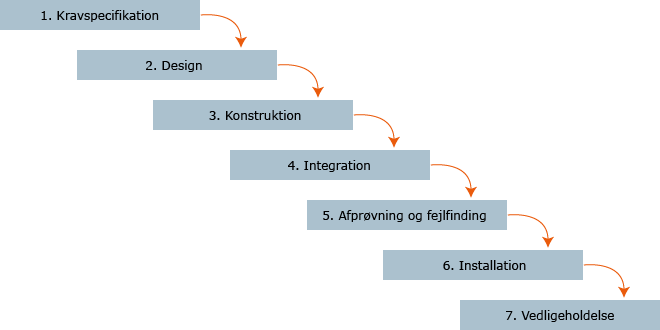
\includegraphics[scale=0.1]{figures/Vandfaldsmodellen}

\section{SCRUM}
Scrum-metoden er en agil udviklingsmetode, som er særligt kendt for dets tilpasning til software udvikling, men også kan bruges i andre projekt sammenhæng og er anerkendt som et agile projektstyringsredskab. Denne metode er, i stedet for faser, opdelt i roller, hvor hver rolle indebære forskelligt ansvar.%\cite{HTL} 
I forhold til andre projektmetoder, har denne ikke nogen leder, men hver person som er en del af Scrum-teamet, har lige meget ansvar. Dog skal der være en såkaldt Scrum Master, hvis ansvar er at have kontakt til Product Owner og sørge for, at Development Teamet er på rette spor med hensyn til udviklingen, tidsplaner med mere, og overholder de forskellige scrum regler der findes. Processen i denne metode, bliver styret ved hjælp af en såkaldt Product Backlog, som indeholder opgaver for hele projektet. Det er så op til Product Owner og Scrum Masteren, at finde ud af hvilke opgaver, der skal laves. For at have et overblik over arbejdsopgaverne, er der lavet såkaldte Sprints, som er arbejdsperioder i et projekt. For hvert Sprint, skal de arbejdsopgaver der er i disse laves færdige, så der opretholdes og overholdes deadlines for projektet. Dette er væsentligt for Scrum metoden, da efter hvert endt Sprint, gerne skal være et produkt, som kan lanceres. En af fordelene ved Scrum er, at der er fokus på at lancere en udgave af produktet kontinuerligt og blive ved med at komme med nye og bedre udgaver af et produkt, så længe det stadig er under udvikling. En af ulemperne ved Scrum kan være, at det er svært for Scrum Masteren at planlægge og strukturere projektet, uden en klar definition på, hvordan det endelige produkt skal se ud, da metoden gør det muligt for Product Owneren at komme med ændringer, som skal implementeres eller ændres i projektet, mellem de forskellige Sprints.%\cite{HTL}

\section{Unified Process (UP)}
Unified Process er også en iterativ og trinvis udviklingsmetode. Metoden består af forskellige iterationer, som hver omhandler deres emne og sætter fokus på bestemte faser i projektet. Faserne er Inception, Elaboration, Construction og Transition, som hver kan være delt op i flere individuelle iterationer alt efter størrelsen på projektet.%\cite{HTL}
Metoden gør det muligt, i forhold til andre iterative metoder som Vandfaldsmodellen, at anvende iterationer, til at analysere, designe, implementere og teste i løbet af projektet, for hele tiden at forbedre og udvikle produktet. I figur XX, kan ses et diagram som illustrere et eksempel på en Iterativ udviklings forløb. En af fordelene ved denne metode er, at efter hver endt iteration, så overlapper de forskellige faser hinanden, så det er muligt at gå tilbage til en fase, som tidligere var afsluttet, og tage det op i en ny iteration. En af ulemperne kan være, at det er meget Use Case drevet / Risiko drevet, da metoden afhænger meget af at man kender alle de risici faktorer, som kan spille ind i løbet af projektet. Hvis ikke alle disse findes til at starte med, kan det have en stor betydning for projektets forløb.%\cite{HTL} 